\chapter{薄板型抗震阻尼器数值模拟分析}
本章对工程应用中常见的四种薄板型抗震阻尼器进行数值仿真分析,对本文所提方法赫林格-赖斯纳变分一致型伽辽金无网格法进行验证,通过对三种不同本质边界条件施加方法得出的应力云图进行分析得出所提方法具有更高的鲁棒性和稳定性。
\section{狭缝阻尼器}
在建筑和工程结构中,振动是一个常见的问题,其可能会导致结构的疲劳破坏等问题,传统方法中通过采用增加结构的刚度或使用液体阻尼器、摩擦阻尼器减小结构的振动响应,然而在传统方法中或多或少的存在有效性不高,经济适用性低等问题。
为了克服传统方法的限制,狭缝阻尼器被引入,
狭缝(slit)阻尼器通过在建筑结构中引入缝隙,进而吸收和耗散振动能量,从而有效减少结构的振动响应,同时slit阻尼器的结构相对简单,由一系列平行的缝隙组成,可以根据具体的需求进行设计和调整,并且狭缝阻尼器通常采用钢材或高性能复合材料制造,具有良好的耐久性和抗腐蚀性能,在工程实践应用中越来越广泛。
图\ref{slit1}为带有slit阻尼器的新型连接体系,梁底部的缝型阻尼器先于主体构件主动塑化,该系统常用于震后修复。
图\ref{slitmsh}为狭缝阻尼器示意图及节点离散示意图,该平面被变形通过对其采用二次基函数,无网格影响域取2.5进行数值求解分析,材料系数分别为杨氏模量$E=2\times 10^{11}$、泊松比$\nu=0.3$。
\begin{figure}[H]
    \centering
    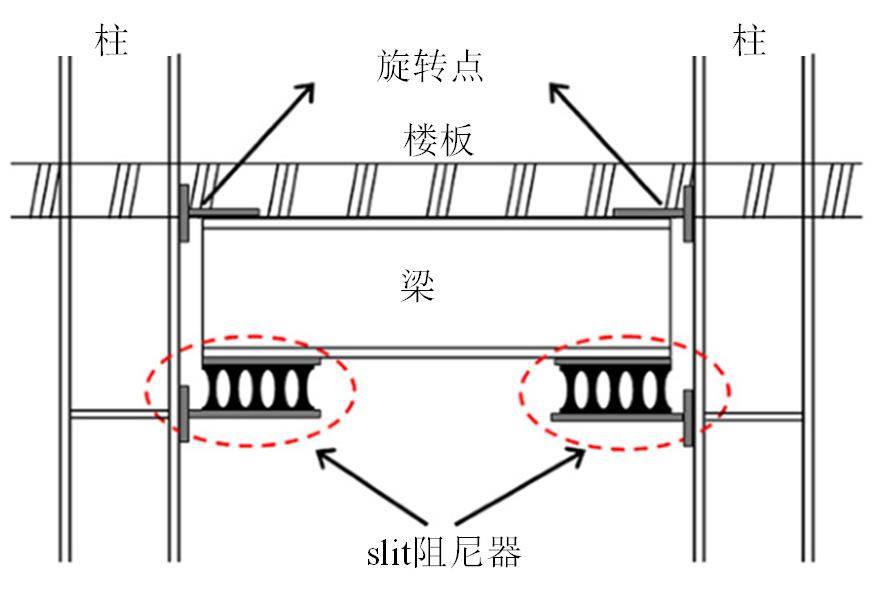
\includegraphics[scale=0.7]{figure/DAMPER/SLIT/1.png}
    \caption{实验装置示意图\cite{oh2009}}\label{slit1}
\end{figure}
% \begin{figure}[H]
%     \centering
%     \begin{subcaptiongroup}
%     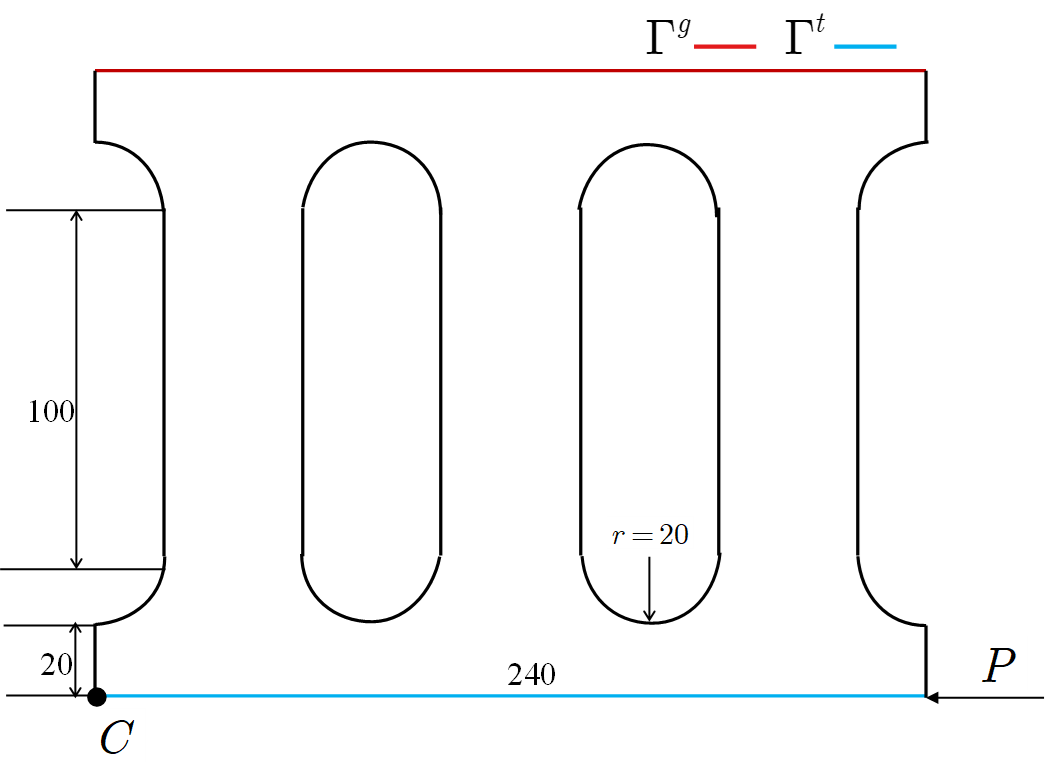
\includegraphics[width=0.49\textwidth]{figure/DAMPER/SLIT/2.png}
%     \phantomcaption\label{slita}
%     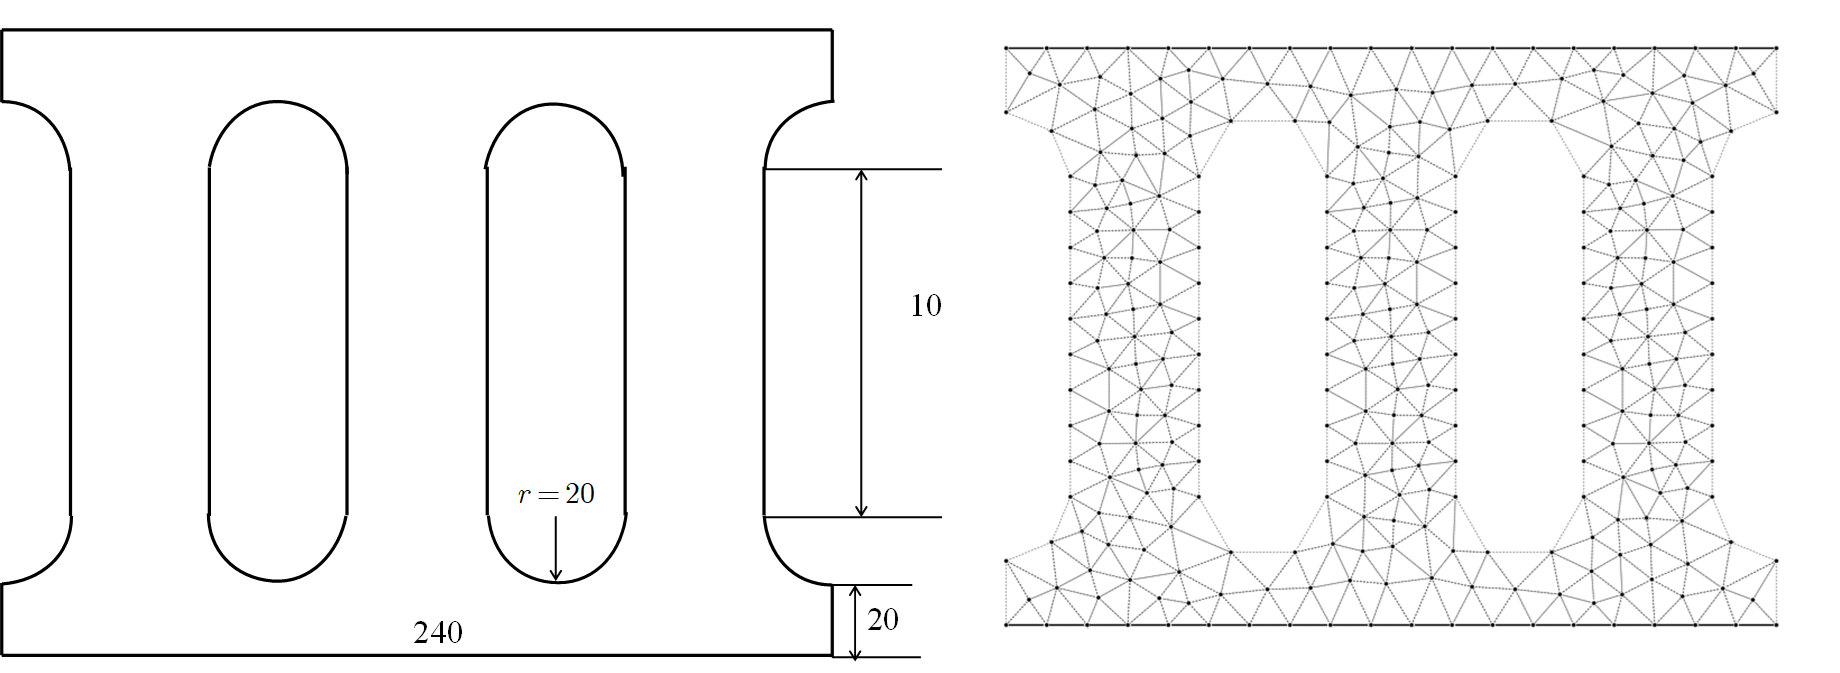
\includegraphics[width=0.49\textwidth]{figure/DAMPER/SLIT/slit damper_msh.png}
%     \phantomcaption\label{slitb}
%     \end{subcaptiongroup}
% \caption{\centering{狭缝阻尼器:\subref{slita}尺寸详图;\subref{slitb}无网格离散模型}}
% \label{slitmsh}
% \end{figure}
% \begin{figure}[H]
%     \centering
%     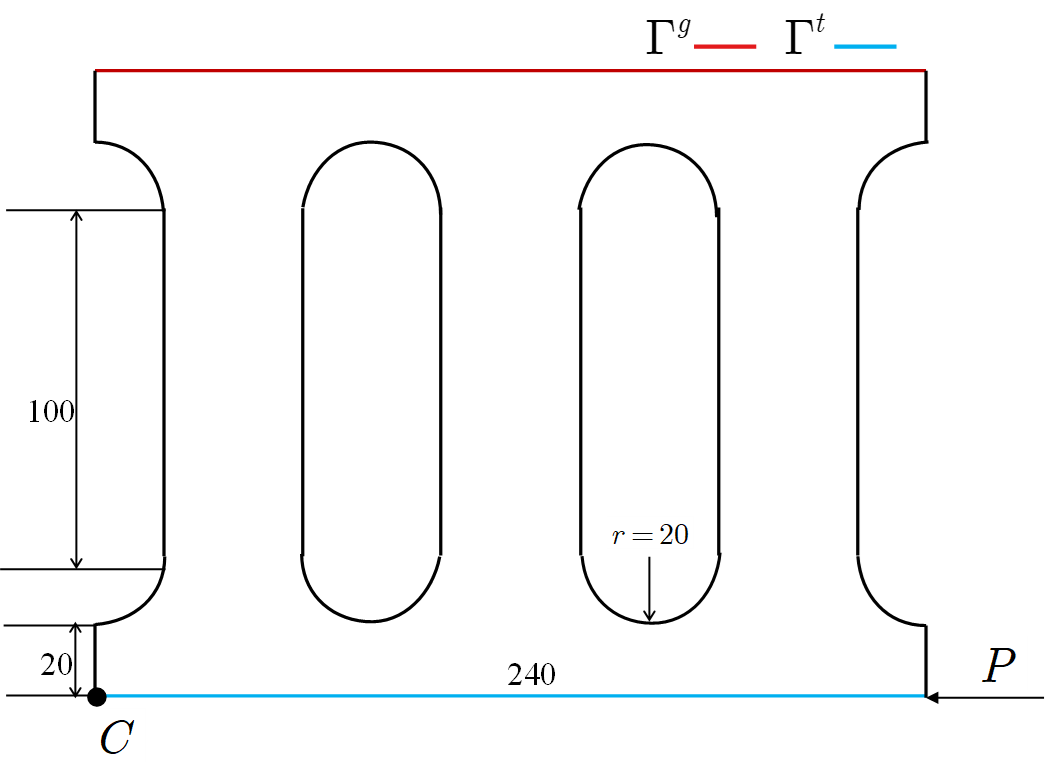
\includegraphics[scale=0.4]{figure/DAMPER/SLIT/2.png}
%     \caption{狭缝阻尼器模型图}\label{slit2}
% \end{figure}
\begin{figure}[H]
    \centering
    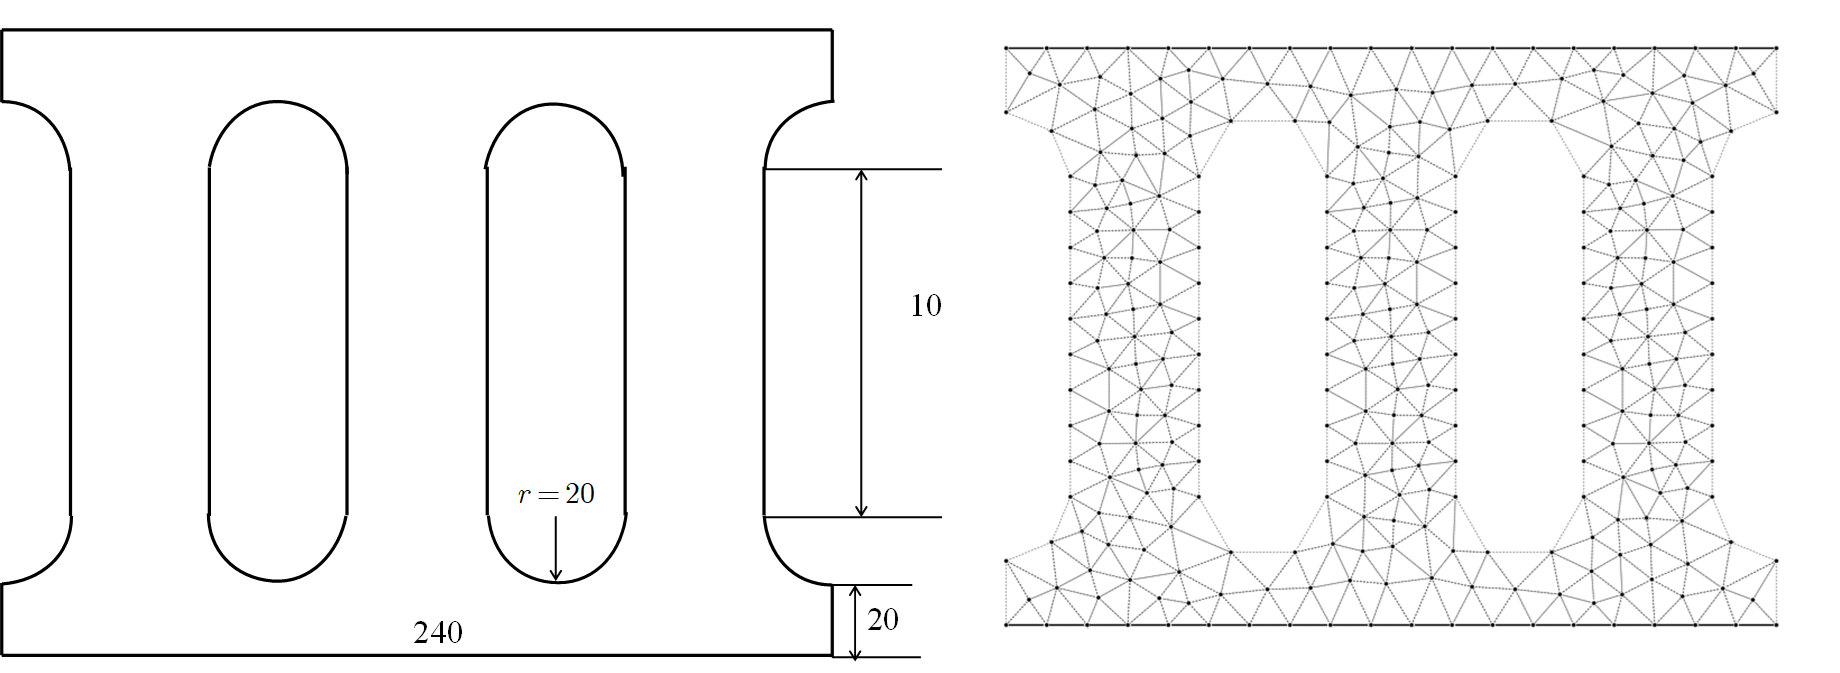
\includegraphics[scale=0.45]{figure/DAMPER/SLIT/slit damper_msh.png}
    \caption{狭缝阻尼器及其无网格离散模型}\label{slitmsh}
\end{figure}
图\ref{slitM}为slit阻尼器三角形板的弯矩应力云图,可以看出Nitsche法和HR法的应力云图没有出现明显的波动现象,相较于罚函数法更稳定。
\begin{figure}[H]
    \centering
        \includegraphics[scale=0.5]{figure/DAMPER/slit/M11.png}
        \includegraphics[scale=0.5]{figure/DAMPER/slit/M12.png}
        \includegraphics[scale=0.5]{figure/DAMPER/slit/M22.png}
    \caption{狭缝阻尼器弯矩云图}\label{slitM}
\end{figure}
\section{蜂窝阻尼器}
蜂窝(Honeycomb)阻尼器通过内部的蜂窝结构和材料的摩擦耗能来提供阻尼效果,相较于传统的阻尼器,蜂窝阻尼器具有更高的阻尼能力,能够有效地减少结构振动幅度,具有高阻尼能力、宽频响特性和轻量化设计地特点,适用于需要控制结构振动地工程应用。
图\ref{Honeycomb1}为带有蜂窝阻尼器的实验装置示意图及模型图。
图\ref{Honeycombmsh}为蜂窝阻尼器尺寸详图及无网格节点离散示意图,该平面内变形进一步通过采用三次基函数,取影响域为3.5进行验证分析。材料系数分别为杨氏模量$E=2\times 10^{11}$、泊松比$\nu=0.3$。
\begin{figure}[H]
    \centering
    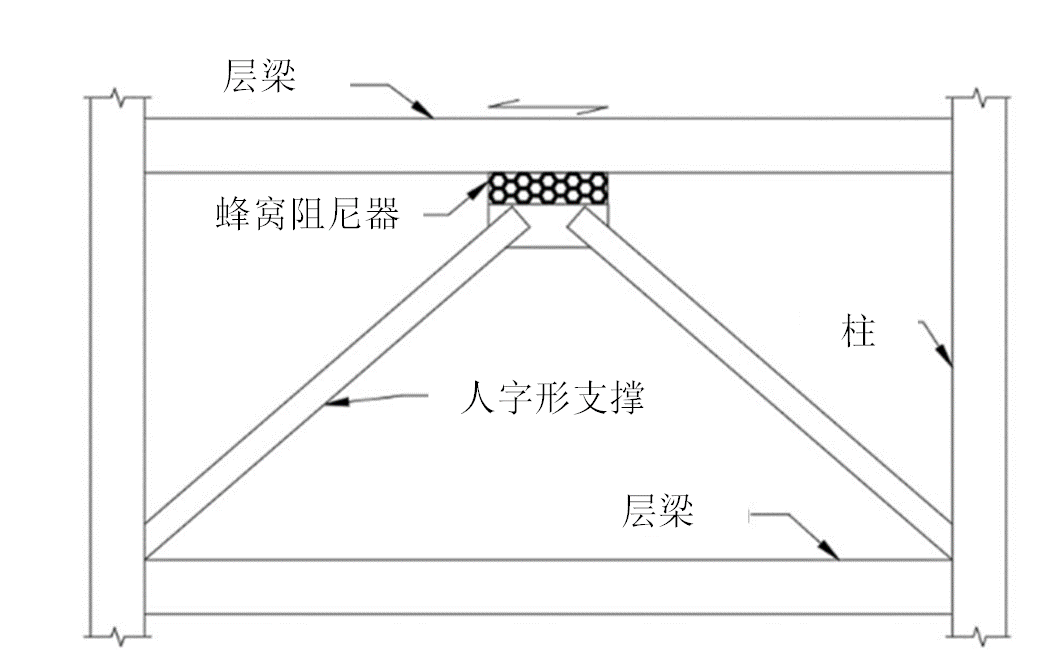
\includegraphics[scale=0.6]{figure/DAMPER/Honeycomb/1.png}
    \caption{实验装置示意图\cite{javanmardi2020}}\label{Honeycomb1}
\end{figure}
% \begin{figure}[H]
%     \centering
%     \begin{subcaptiongroup}
%     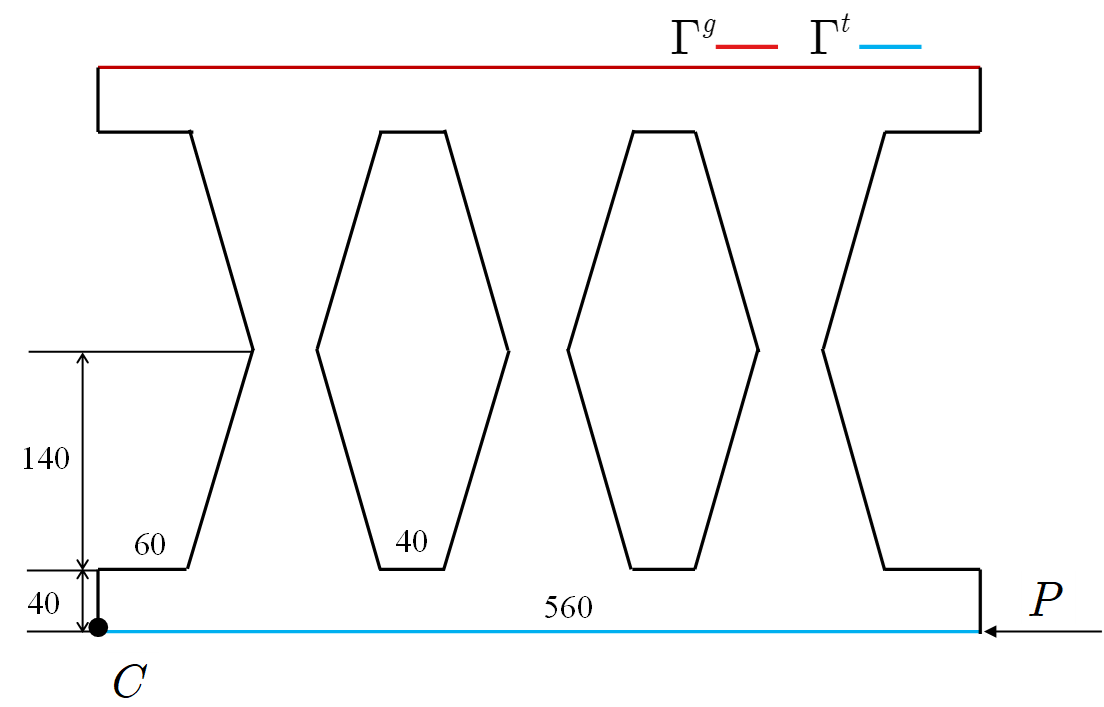
\includegraphics[width=0.49\textwidth]{figure/DAMPER/Honeycomb/2.png}
%     \phantomcaption\label{Honeycomba}
%     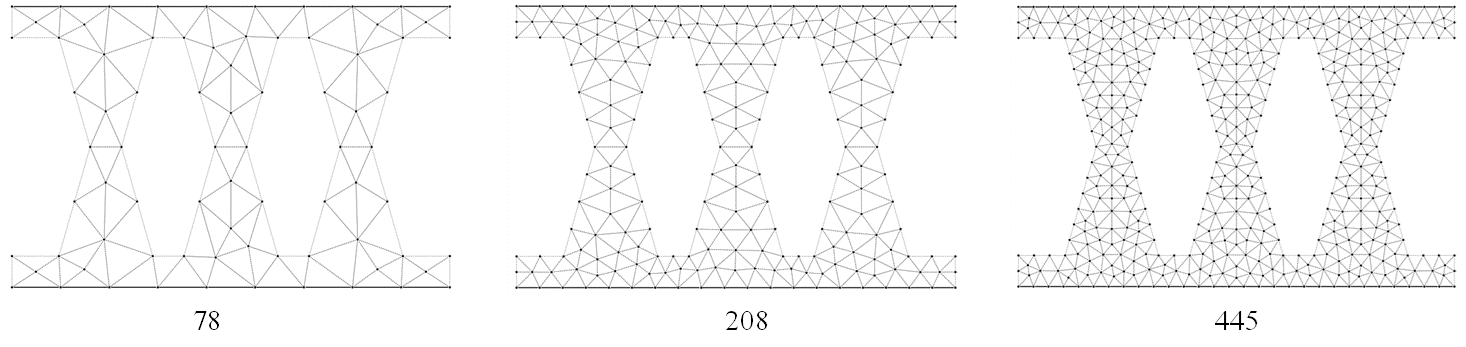
\includegraphics[width=0.49\textwidth]{figure/DAMPER/Honeycomb/honeycomb_damper_msh.png}
%     \phantomcaption\label{Honeycombb}
%     \end{subcaptiongroup}
% \caption{\centering{蜂窝阻尼器:\subref{Honeycomba}尺寸详图;\subref{Honeycombb}无网格离散模型}}
% \label{Honeycombamsh}
% \end{figure}
% \begin{figure}[H]
%     \centering
%     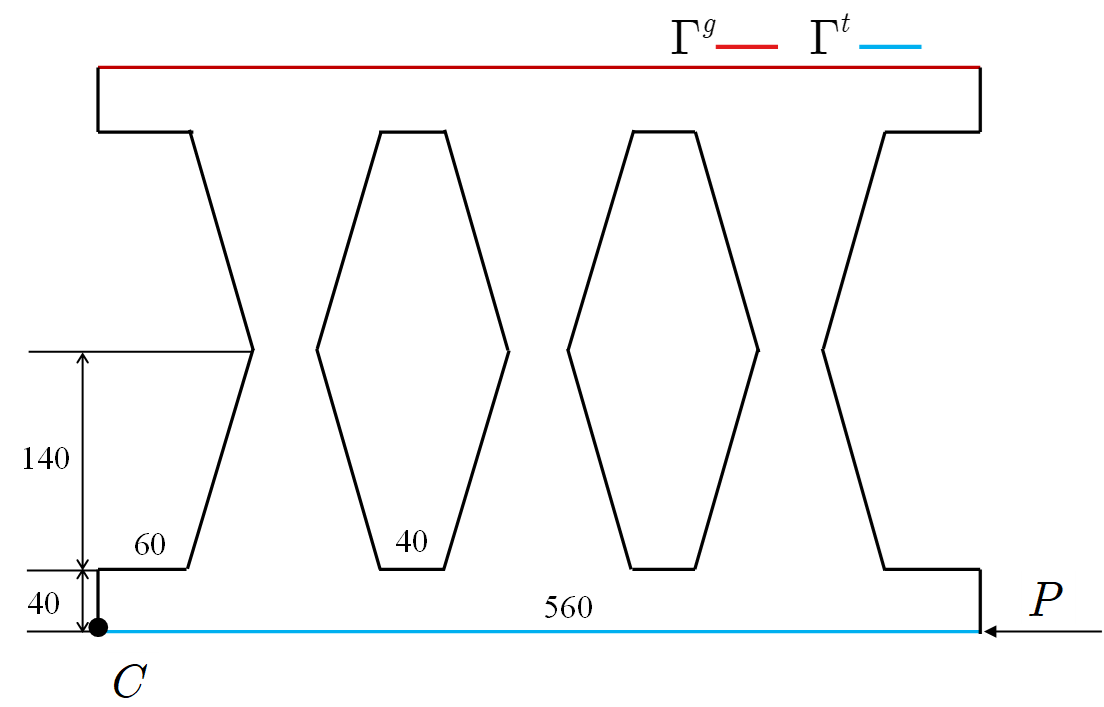
\includegraphics[scale=0.6]{figure/DAMPER/Honeycomb/2.png}
%     \caption{蜂窝阻尼器模型图}\label{Honeycomb2}
% \end{figure}
\begin{figure}[H]
    \centering
    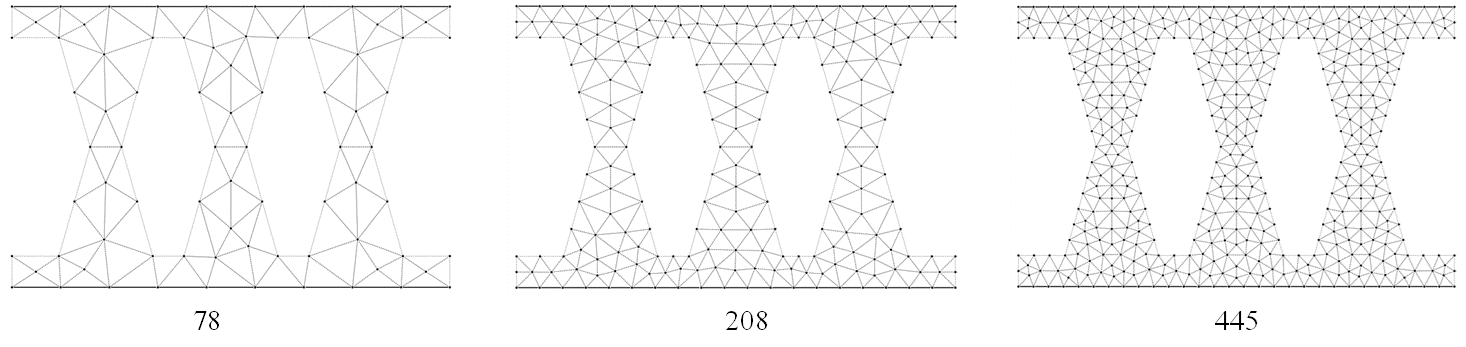
\includegraphics[scale=0.45]{figure/DAMPER/Honeycomb/honeycomb_damper_msh.png}
    \caption{蜂窝阻尼器及其无网格离散模型}\label{Honeycombmsh}
\end{figure}
图\ref{HoneycombM}是受到平面内变形的蜂窝阻尼器的应力云图,从图中可以看出所提方法HR法有着更稳定的数值计算结果。
\begin{figure}[H]
    \centering
        \includegraphics[scale=0.5]{figure/DAMPER/Honeycomb/M11.png}
        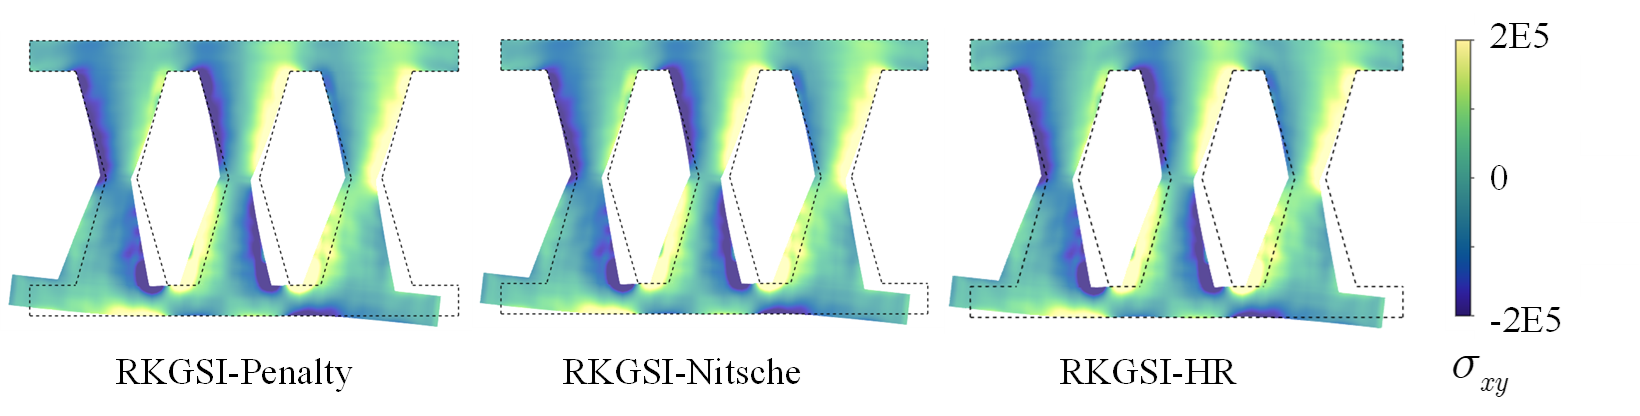
\includegraphics[scale=0.5]{figure/DAMPER/Honeycomb/M12.png}
        \includegraphics[scale=0.5]{figure/DAMPER/Honeycomb/M22.png}
    \caption{蜂窝阻尼器弯矩云图}\label{HoneycombM}
\end{figure}
\section{ADAS阻尼器}
ADAS阻尼器是一种基于能量耗散原理的被动控制装置,通过在结构中引入附加的阻尼力来吸收和耗散结构的振动能量,能够有效地减小结构地的振动幅值和振动周期,从而显著改善结构的振动响应,
并且ADAS阻尼器的设计相对简单,通常由一块或多块金属材料制成,安装简易、价格低廉,是一种在结构工程中广泛应用于减震和控制结构的被动控制装置。
图\ref{ADAS1}为ADAS阻尼器与裸框架实验装置示意图。
如图\ref{ADASmsh}所示,ADAS阻尼器中的上端部分设为简支固定,对下端施加$P=100000$,厚度设为5,ADAS阻尼器钢板的材料系数分别为杨氏模量$E=2\times 10^{11}$、泊松比$\nu=0.3$。数值分析通过采用三次基函数,取其影响域为3.5进行求解。
\begin{figure}[H]
    \centering
    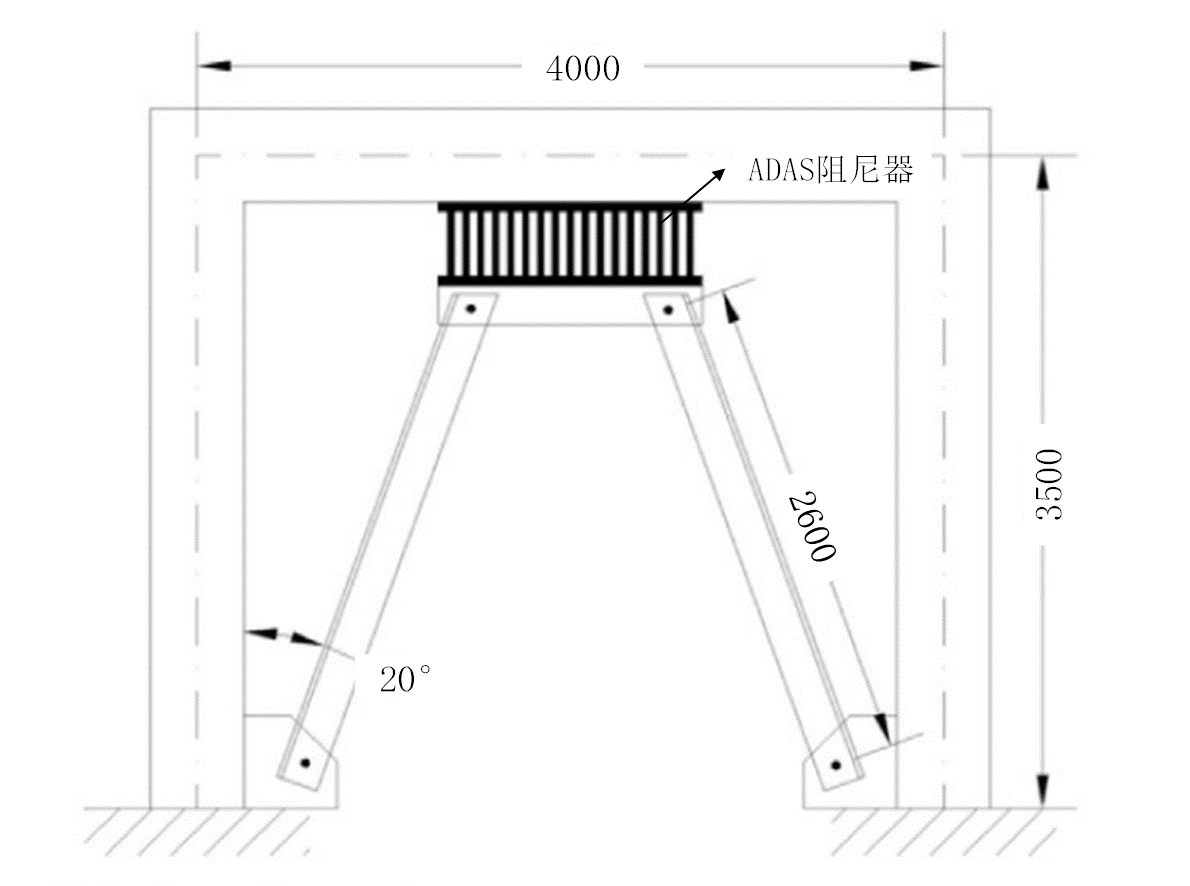
\includegraphics[scale=0.6]{figure/DAMPER/ADAS/1.png}
    \caption{实验装置示意图\cite{basu2016}}\label{ADAS1}
\end{figure}
% \begin{figure}[H]
%     \centering
%     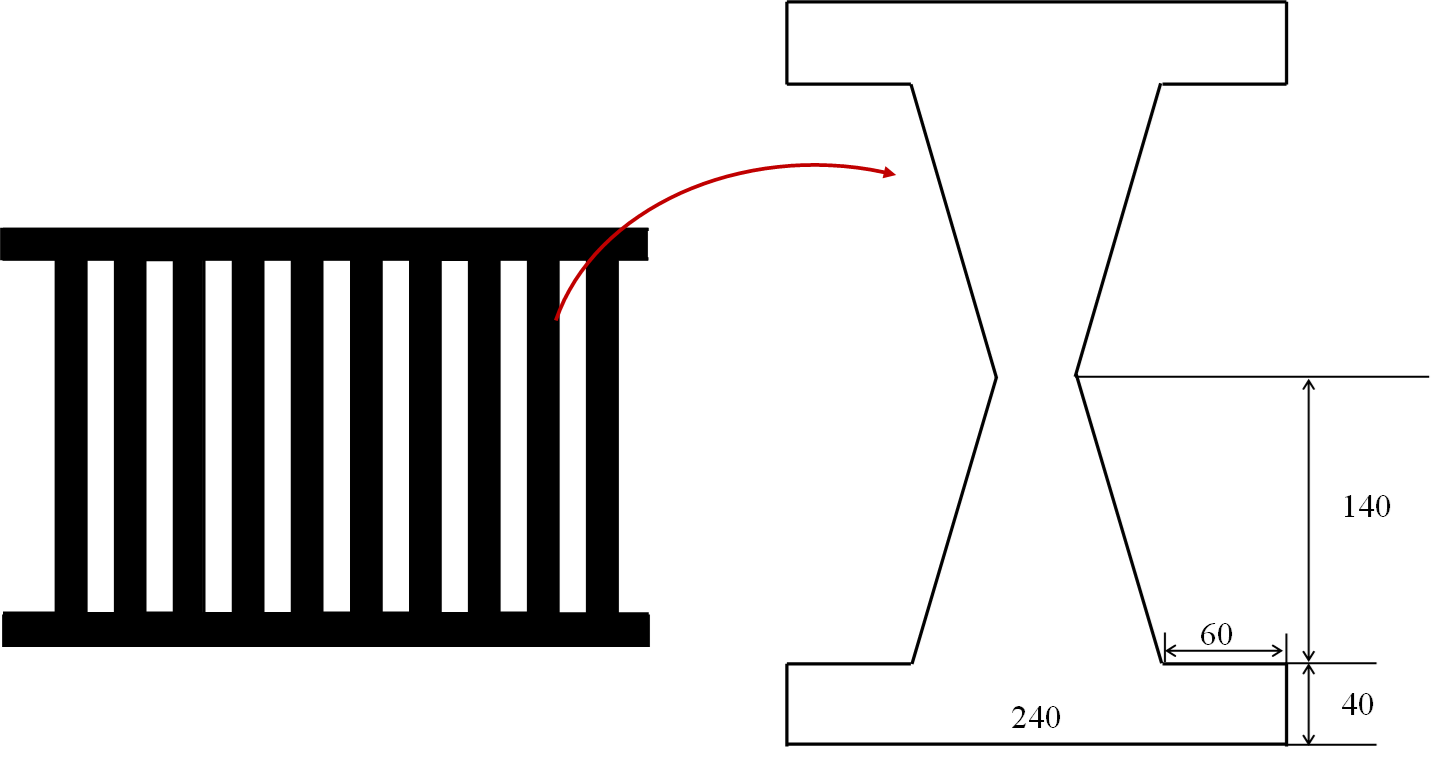
\includegraphics[scale=0.5]{figure/DAMPER/ADAS/2.png}
%     \caption{ADAS阻尼器}\label{ADAS2}
% \end{figure}
\begin{figure}[H]
    \centering
    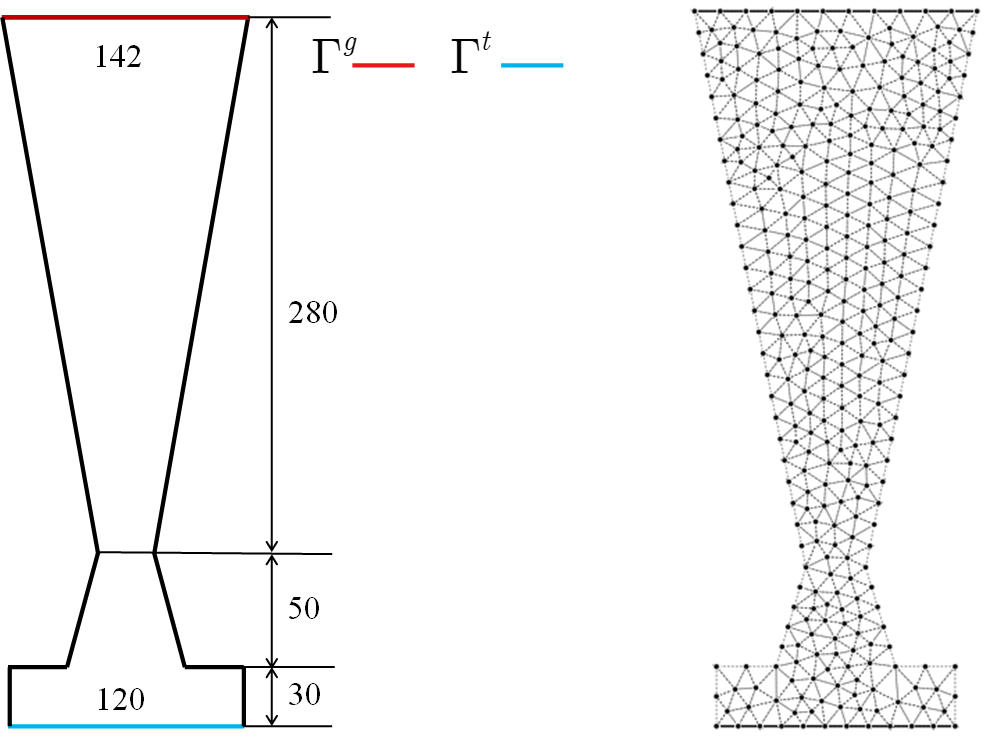
\includegraphics[scale=0.5]{figure/DAMPER/ADAS/ADAS damper_msh.png}
    \caption{ADAS阻尼器及其无网格离散模型}\label{ADASmsh}
\end{figure}
图\ref{ADASM}为ADAS阻尼器受到平面外变形的弯矩云图,从图中可以看出罚函数法和Nitsche法以及所提方法HR法对比,出现明显的波动现象,Nitsche法和HR法拥有几乎相同的弯矩应力,但Nitsche法的计算效率低于HR法,因此所提方法HR法在计算薄板型ADAS阻尼器不仅提高计算精度还有效提高计算效率。
\begin{figure}[H]
    \centering
        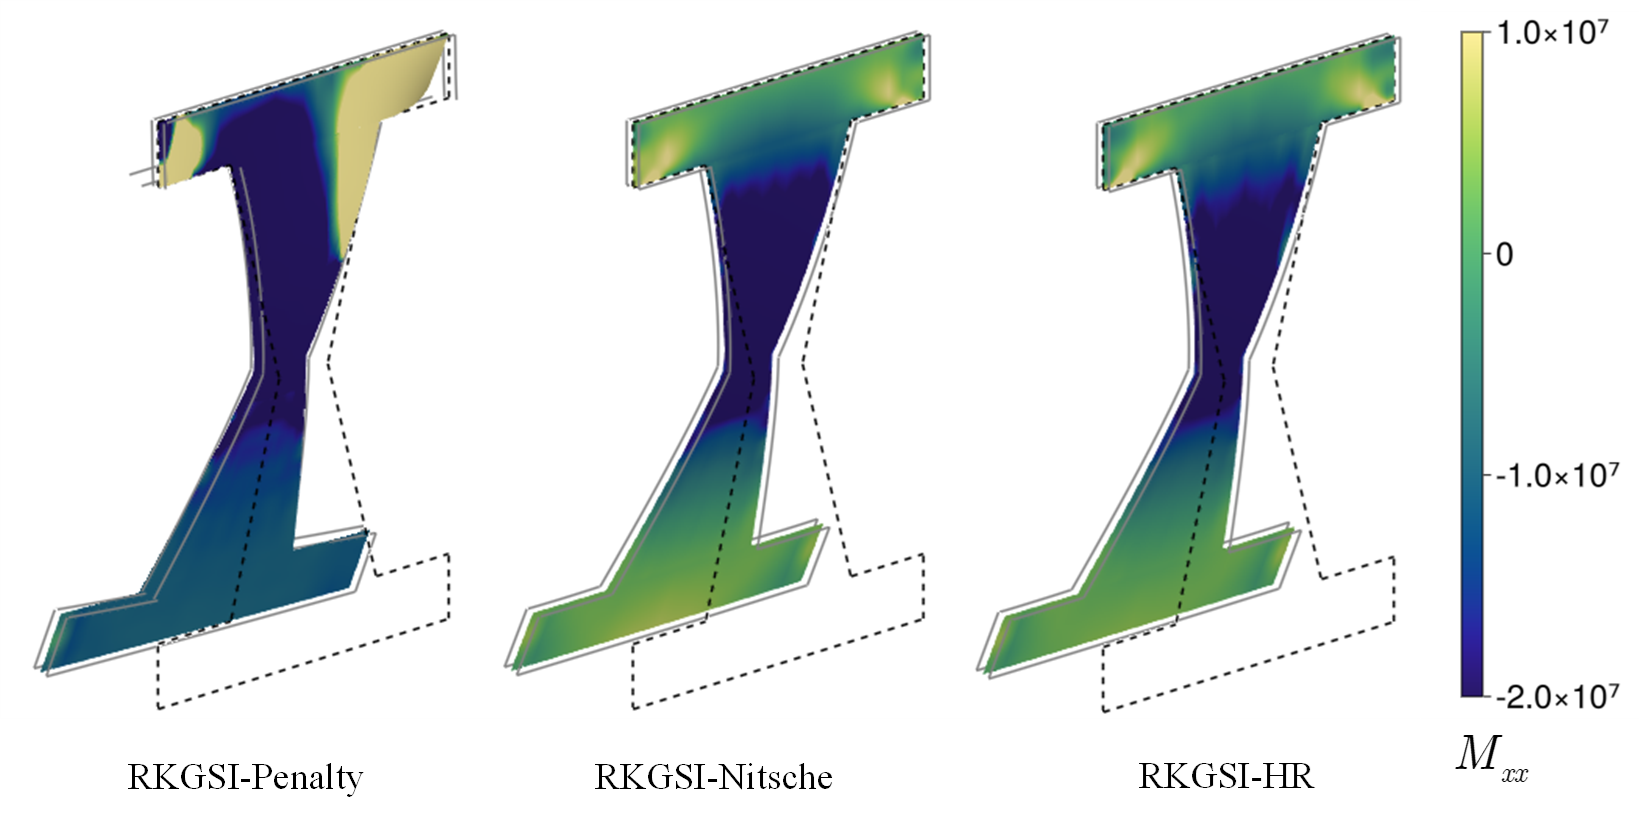
\includegraphics[scale=0.5]{figure/DAMPER/ADAS/M11.png}
        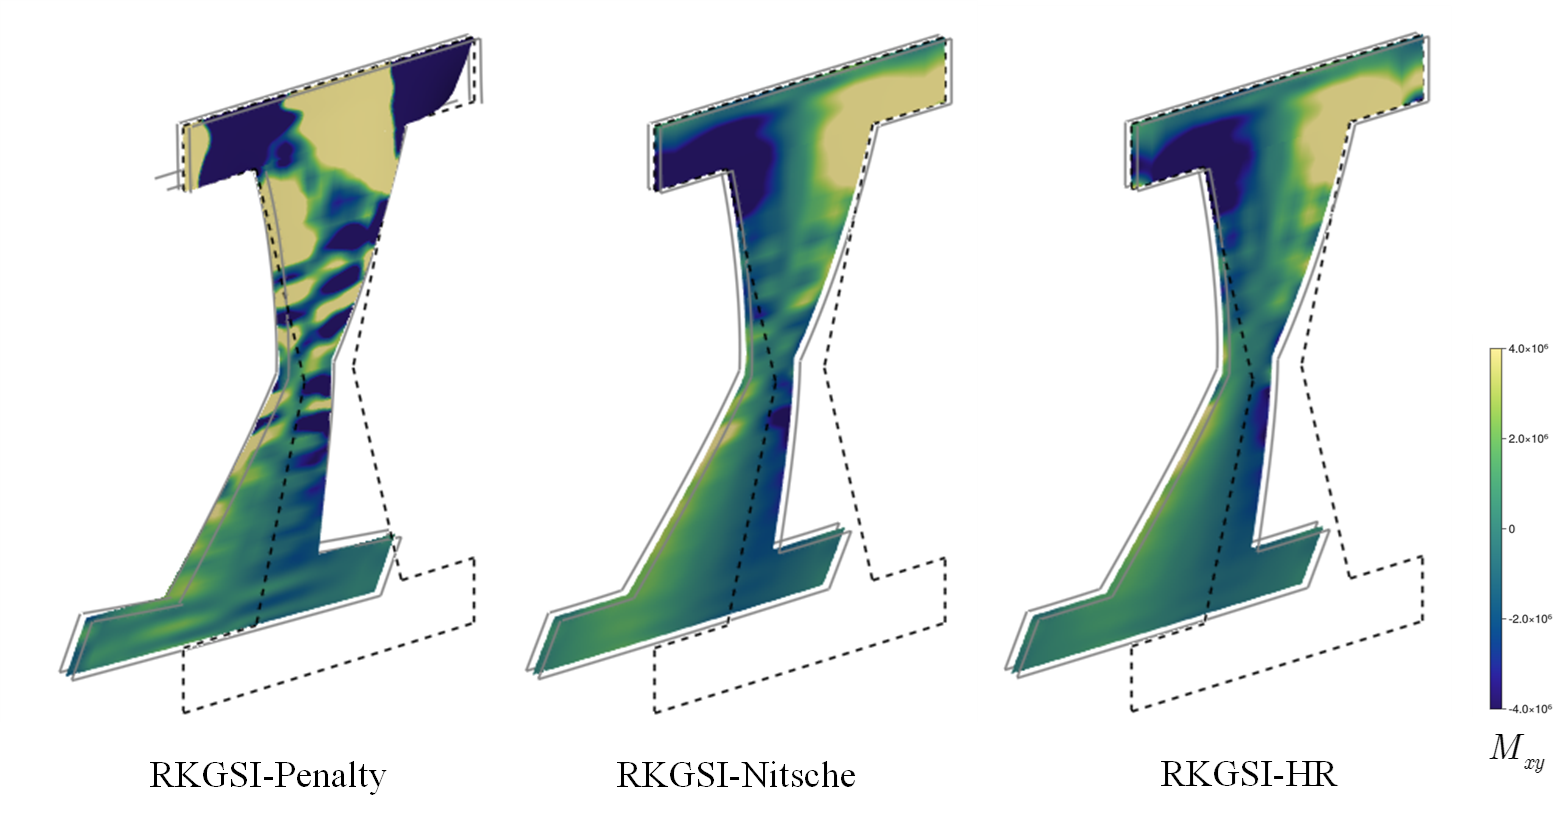
\includegraphics[scale=0.5]{figure/DAMPER/ADAS/M12.png}
        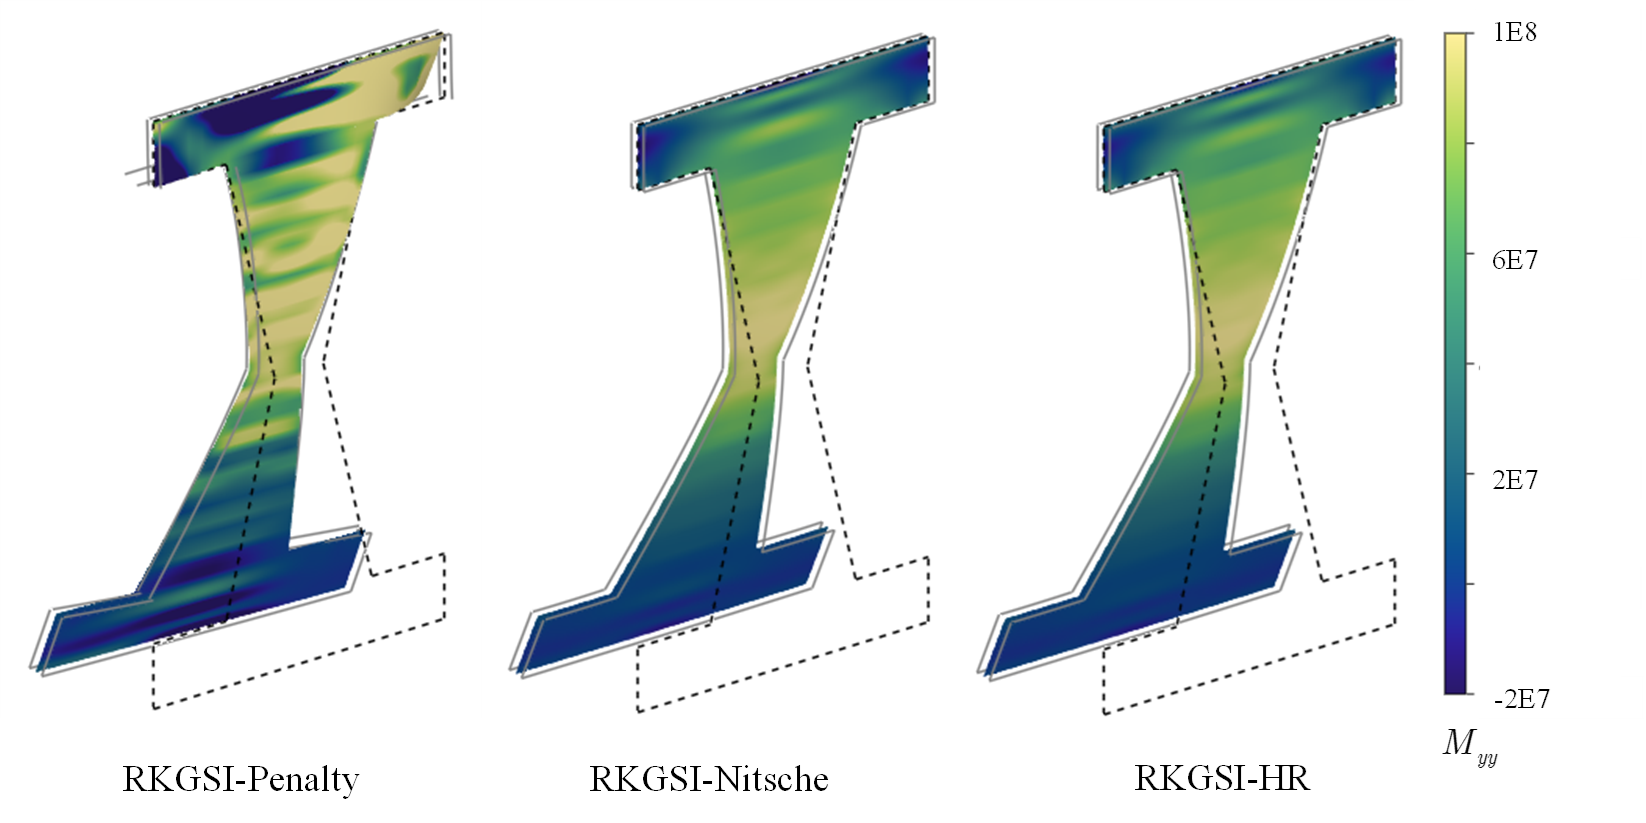
\includegraphics[scale=0.5]{figure/DAMPER/ADAS/M22.png}
    \caption{ADAS阻尼器弯矩云图}\label{ADASM}
\end{figure}
\section{TADAS阻尼器}
ADAS阻尼器的适用性有限,一旦发生横向变形,板将受到张力的影响,导致ADAS的“颈部”X部分容易失效,导致该设备的有效性降低。
为了改善ADAS阻尼器的缺点,三角板(TADAS)阻尼器被开发出来,相较于传统的ADAS阻尼器具有不受重力荷载的影响,但构造比ADAS阻尼器复杂。
图\ref{TADAS1}为一个带有TADAS阻尼器的实验装置\cite{mohammadi2017},为常在道路、住房和城市中心建造的一层框架大比例模型,
该框架高3000,跨度4000,框架柱采用标准的双IPE180型钢材,梁的工字截面由三块$4000\times200\times12$的钢板连续焊接而成。支撑体系统一采用双$100\times100\times20$角度,柱基座使用销连接。
如图\ref{TADASmsh}所示,ADAS阻尼器通过刚性焊接到顶板,下端简单连接到一个开槽底板,ADAS阻尼器中的三角形板的上端设为简支固定,下端施加$P=100000$的力,材料系数为杨氏模量$E=2\times 10^{11}$、泊松比$\nu=0.3$。
通过如图所示的节点进行离散,采用四次基函数,取其影响域为4.5进行求解。
\begin{figure}[H]
    \centering
    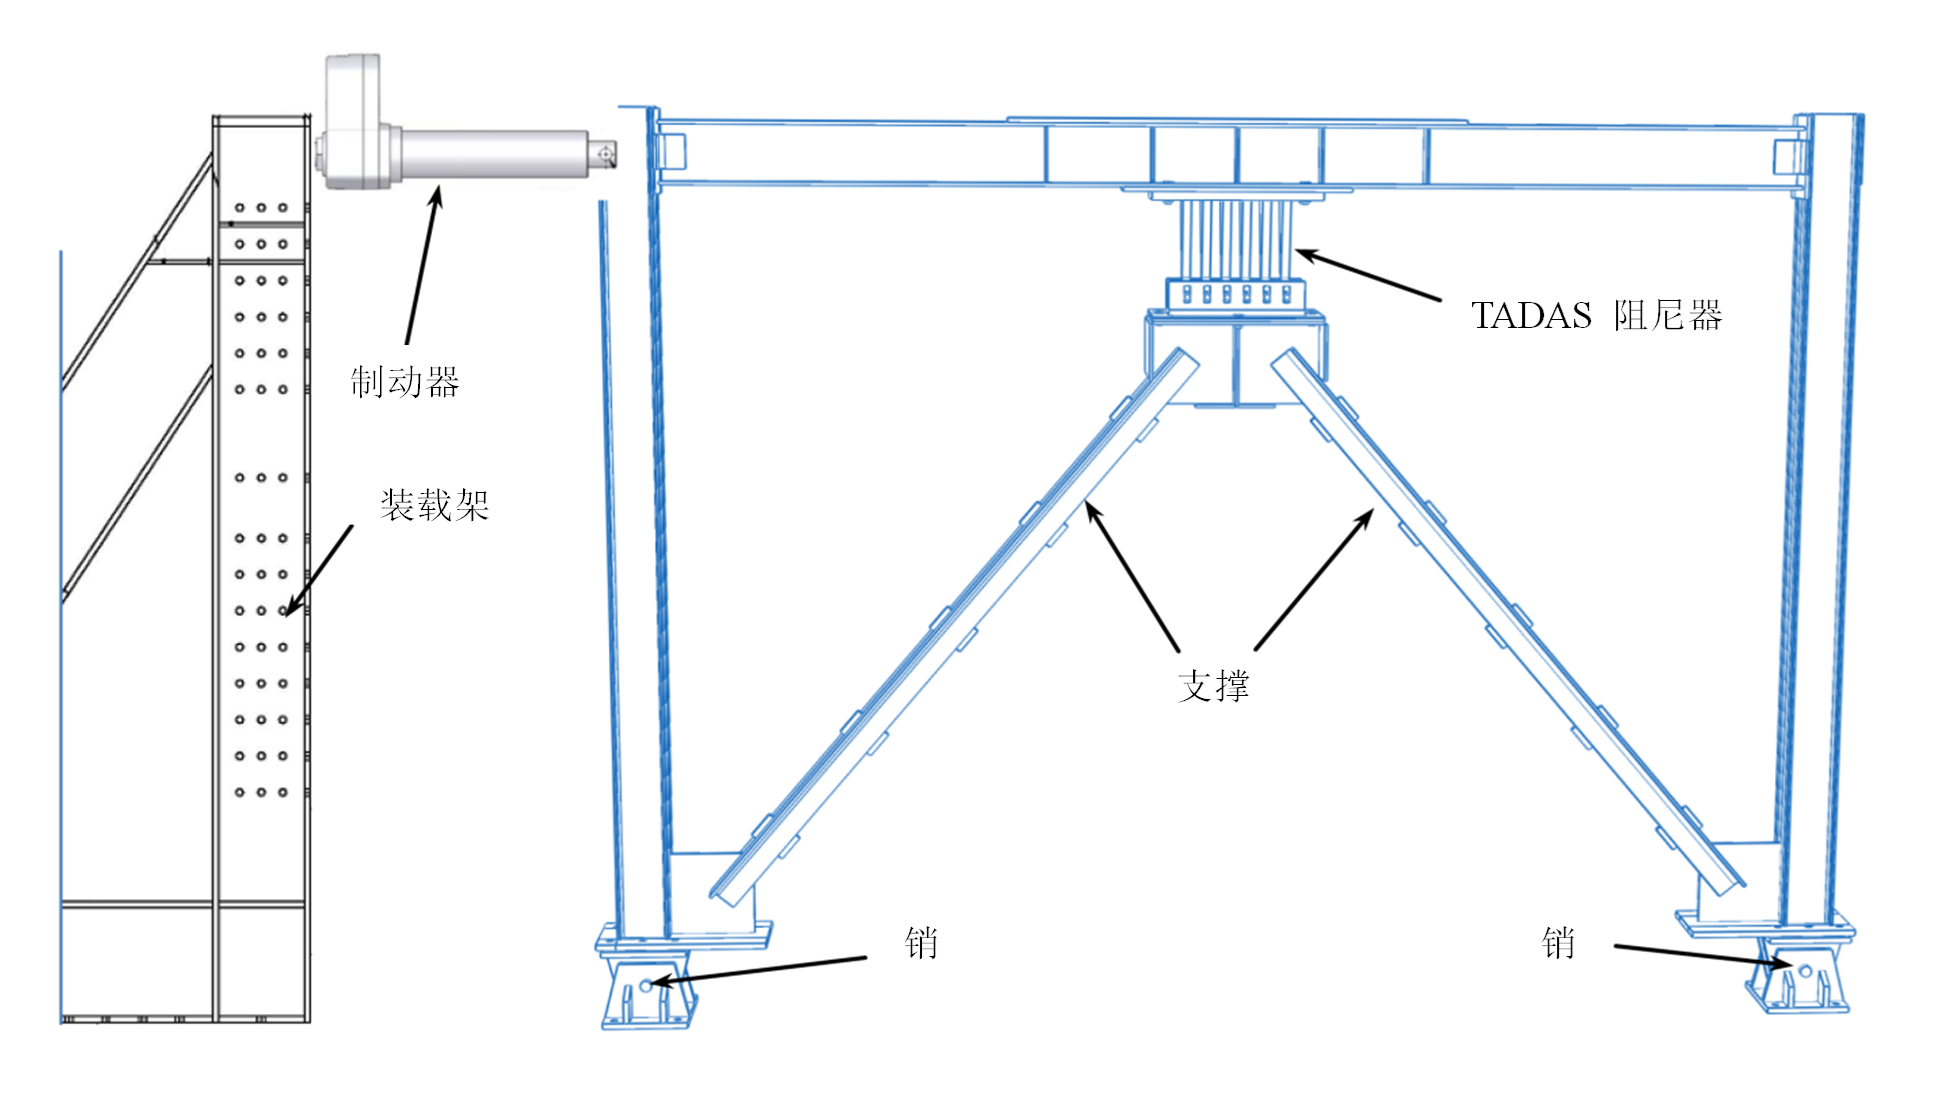
\includegraphics[scale=0.4]{figure/DAMPER/TADAS/1.png}
    \caption{实验装置示意图\cite{mohammadi2017}}\label{TADAS1}
\end{figure}
% \begin{figure}[H]
%     \centering
%     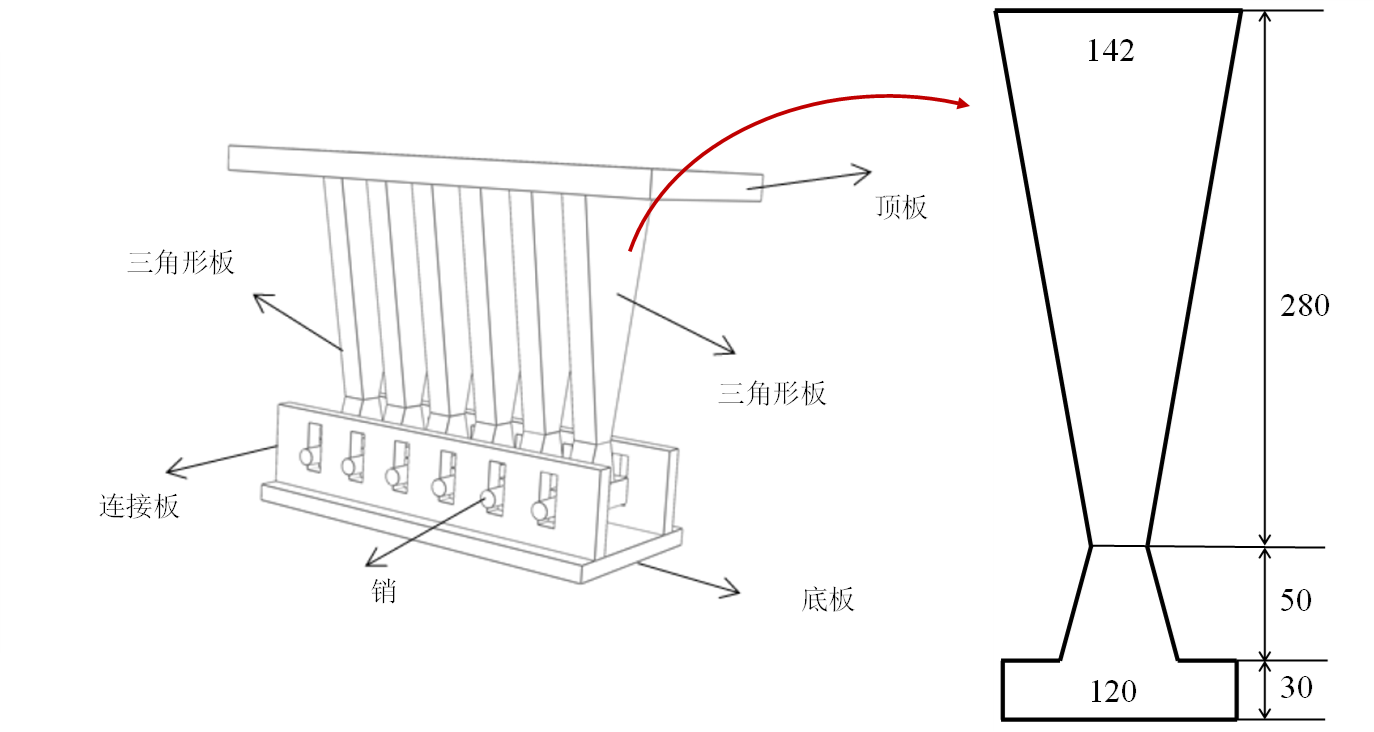
\includegraphics[scale=0.6]{figure/DAMPER/TADAS/2.png}
%     \caption{TADAS示意图\cite{mohammadi2017}}\label{TADAS2}
% \end{figure}
\begin{figure}[H]
    \centering
    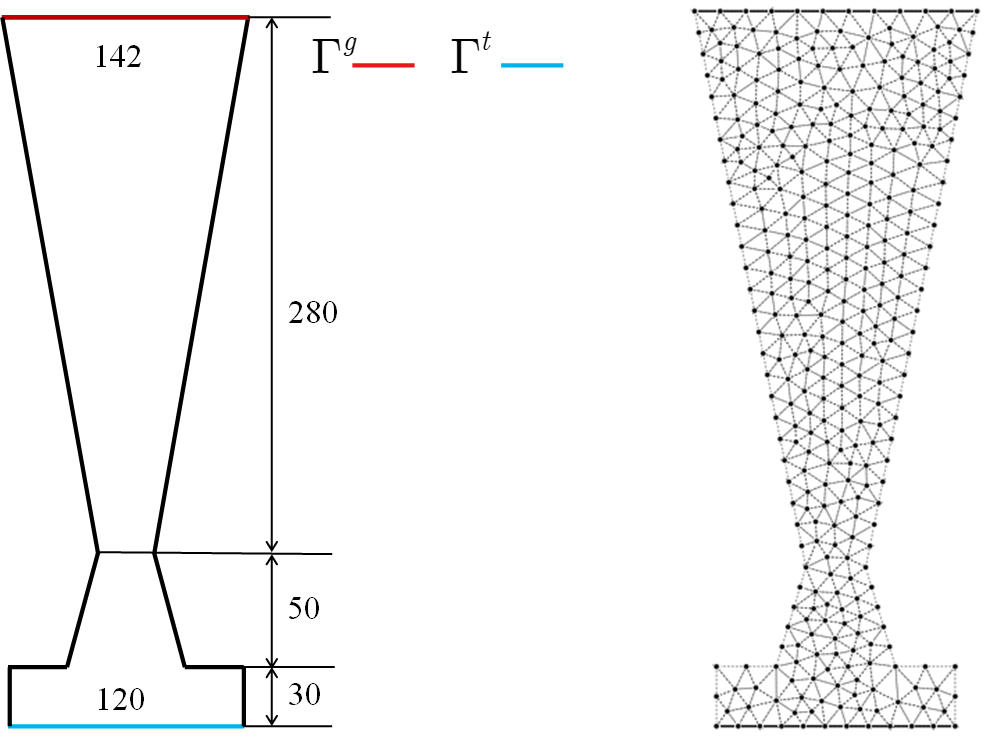
\includegraphics[scale=0.6]{figure/DAMPER/TADAS/TADAS dampers_msh.png}
    \caption{TADAS阻尼器及其无网格离散模型}\label{TADASmsh}
\end{figure}
图\ref{TADASM}为TADAS阻尼器三角形板的弯矩应力云图,从弯矩云图可以看出相较于罚函数法(RKGSI-Penalty),所提方法(RKGSI-HR)拥有更稳定的弯矩云图,有效提高计算精度。
\section{小结}
阻尼器在工程应用中起着减震、减振、控制共振等重要应用,因钢、铝合金等金属材料具有高强度和刚性,能够承受较大的负荷并提供稳定的阻尼效果,使得目前阻尼器的原材料多为金属材料。
在本章中首先对实际工程算例中4种常见的薄板型抗震阻尼器进行介绍,随后分别通过采用不同的本质边界条件施加方法-罚函数法、Nitsche法和本文所提赫林格-赖斯纳变分一致性伽辽金无网格法进行数值仿真分析,通过应力分析云图进一步验证了所提方法在运用实际工程算例中的有效性,为实际工程中实体和薄板模型提供了一种稳定、可靠和高效的数值仿真工具。
\begin{figure}[H]
    \centering
        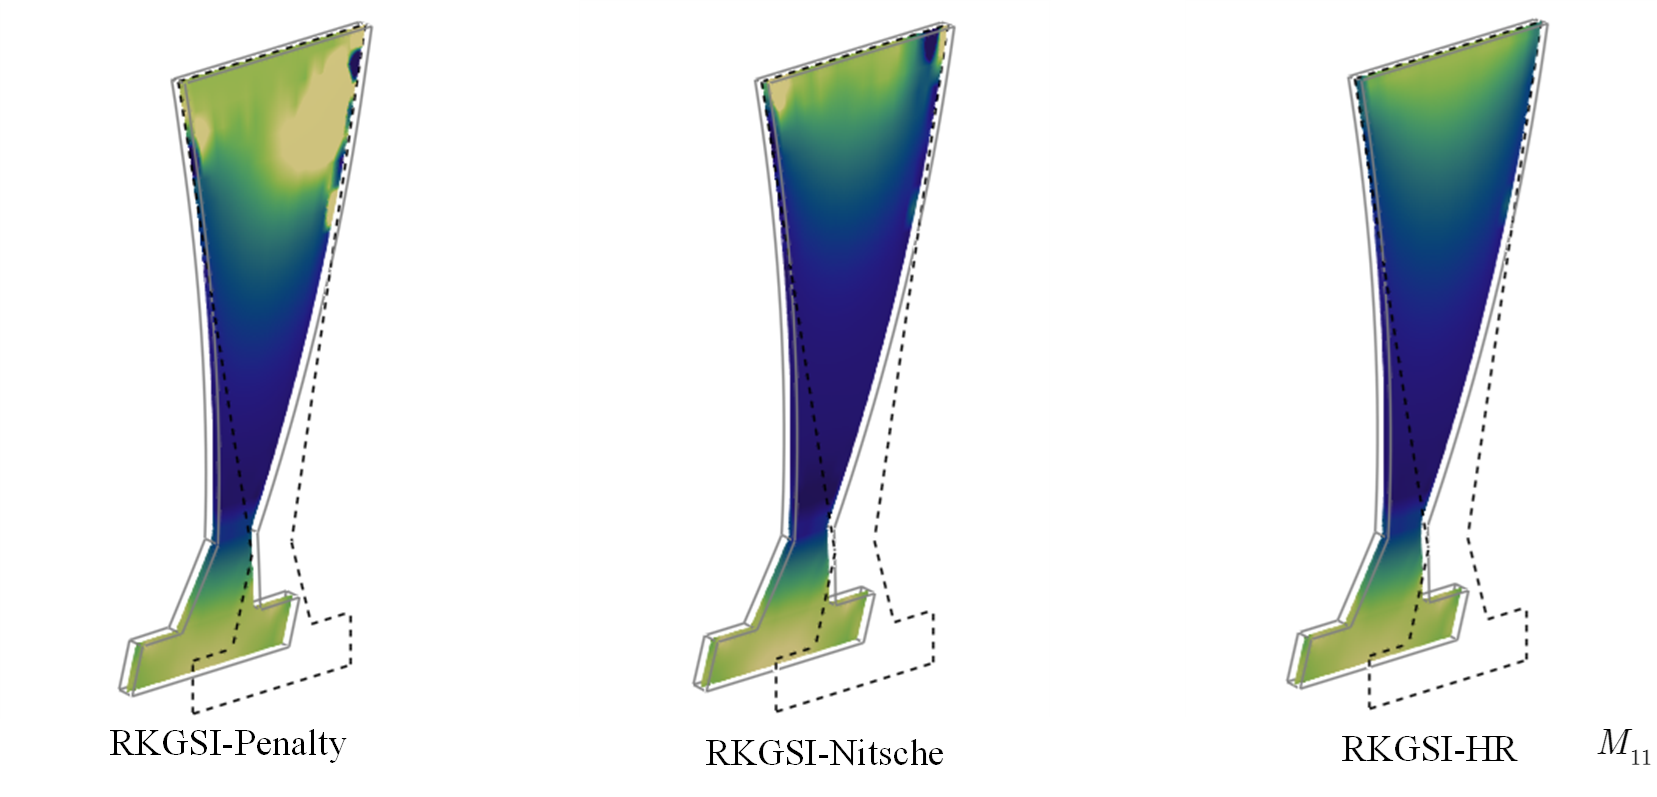
\includegraphics[scale=0.5]{figure/DAMPER/TADAS/M11.png}
        \includegraphics[scale=0.5]{figure/DAMPER/TADAS/M12.png}
        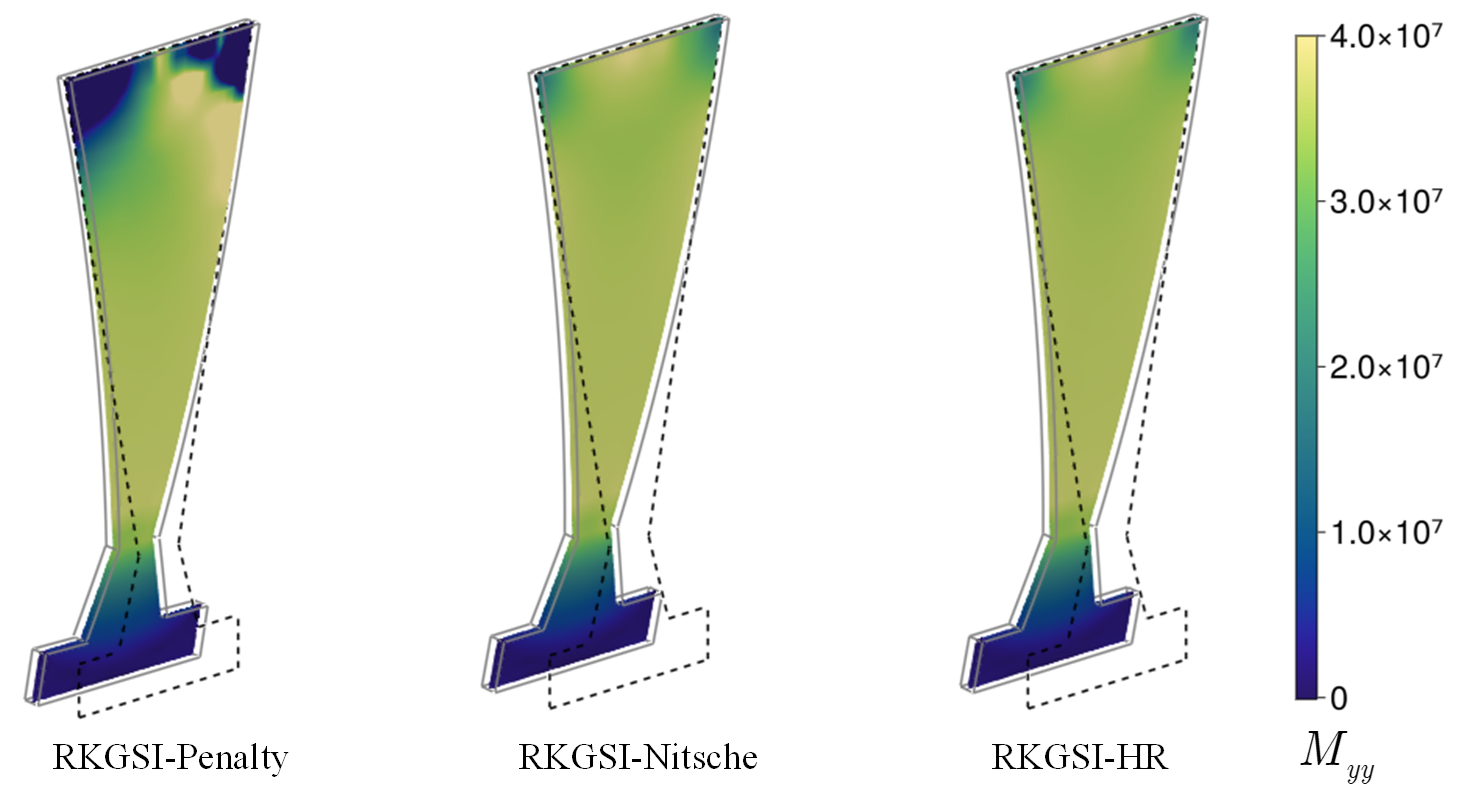
\includegraphics[scale=0.5]{figure/DAMPER/TADAS/M22.png}
    \caption{TADAS阻尼器弯矩云图}\label{TADASM}
\end{figure}


